\chapter{Link--Discovery--Framework}

\section{Modell des Weltausschnittes}
\label{world_model}

Der folgende Abschnitt beschäftigt sich mit der Modellierung des im Rahmen dieser Arbeit verwendeten Weltausschnittes. 

\begin{figure}
\centering
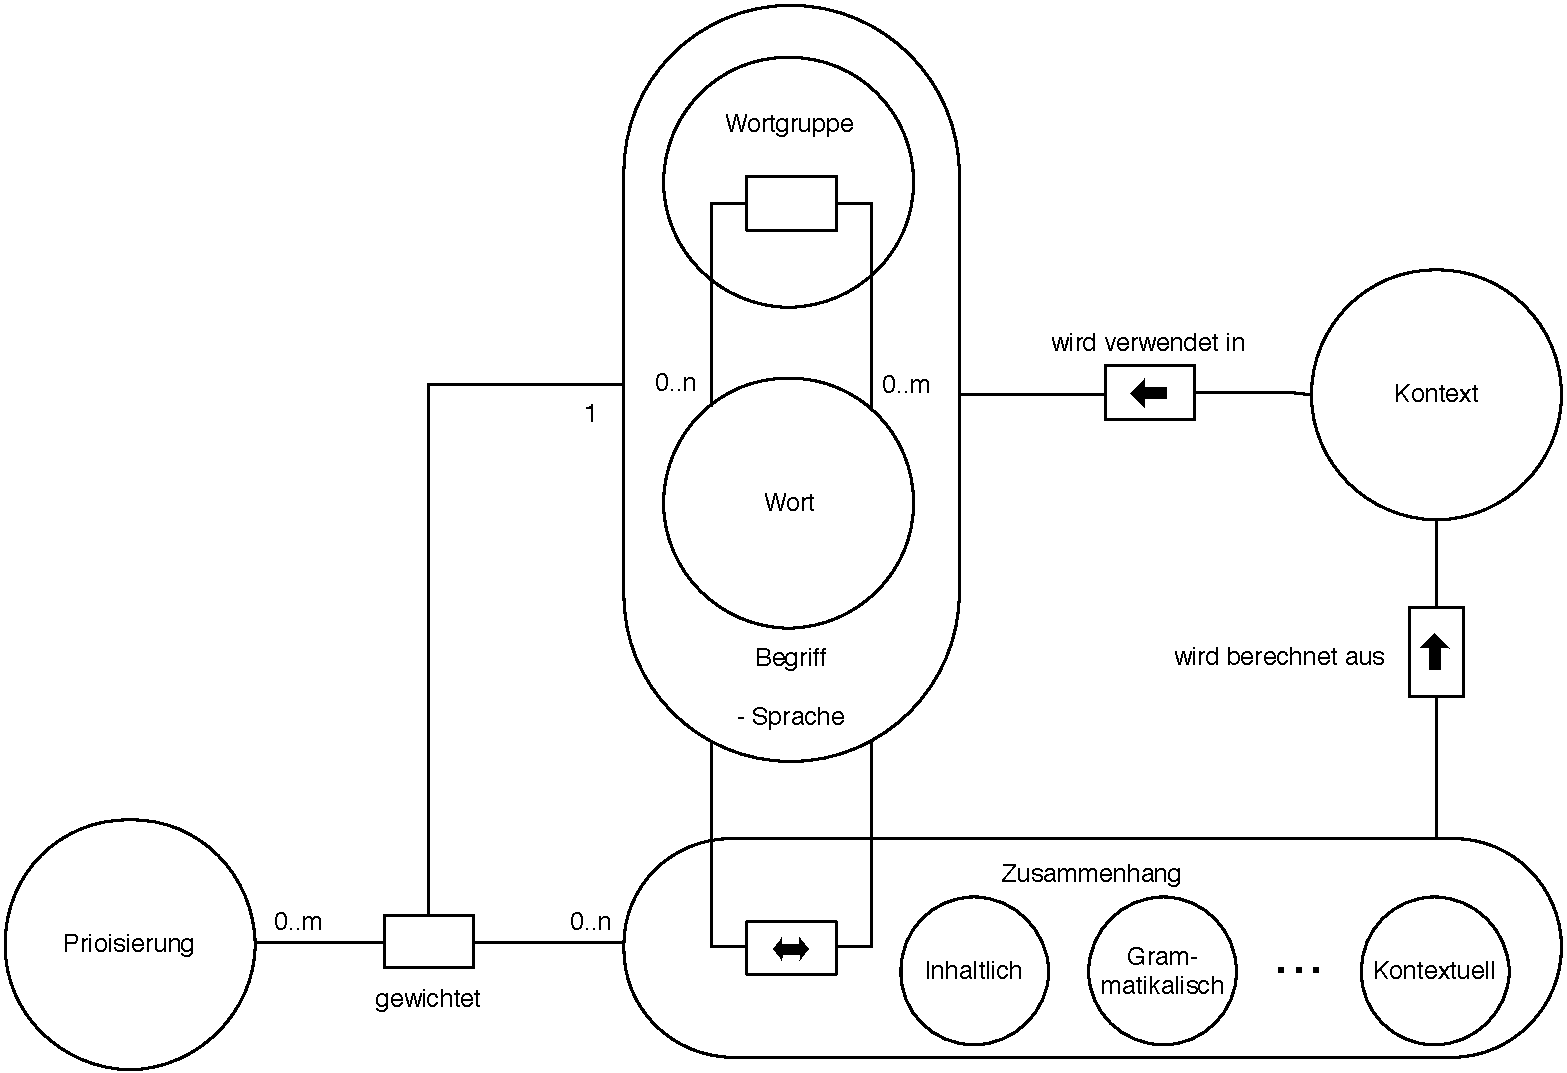
\includegraphics[width=\textwidth]{abstract_world_model}
\caption{Abstraktes Modell des Weltausschnittes}
\label{fig:world_model}
\end{figure}

Abbildung \ref{fig:world_model} zeigt das Modell als Entity--Relationship--Diagramm.

Zentrale Entität ist des Modelles der \emph{Begriff}. Ein Begriff repräsentiert ein Einzelwort oder eine Wortgruppe in einer bestimmten Sprache. Dies berücksichtigt den Umstand, dass Wörter in mehreren Sprachen vorkommen können, jedoch verschiedene Bedeutungen besitzen können. Wortgruppen können aus beliebig vielen Einzelwörtern zusammengesetzt sein. Mit Hilfe der Link Discovery sollen zwischen diesen Begriffen verschiedenartige \emph{Zusammenhänge} gefunden werden.

Ein Zusammenhang besteht immer zwischen genau zwei Begriffen und besitzt einen bestimmten \emph{Typ}. Der Typ bezeichnet die Art des Zusammenhangs zwischen diesen beiden Begriffen. Beispiele für Zusammenhangsarten sind inhaltliche Zusammenhänge wie Synonyme, grammatikalische Zusammenhänge wie Wortformen und Grundformen oder kontextuelle Zusammenhänge, die sich aus der Verwendung des Begriffes ergeben. Dabei kann ein Zusammenhang abhängig vom Typ Attribute besitzen, die den Zusammenhang genauer spezifizieren. Dies kann beispielsweise ein Gewicht des Zusammenhangs sein, dass die Wichtigkeit gegenüber anderen Beziehungen gleichen Typs angibt.

Je nach Nutzungsform der Daten wird unter Umständen eine andere Sicht auf die Beziehungen benötigt. Eine \emph{Prioisierung} stellt eine Gewichtung der Beziehungen eines Begriffes nach Typ dar. Sie teilt jeder Zusammenhangsart ein Gewicht relativ zu den anderen Arten zu. Somit werden durch die Prioisierung bestimmte Zusammenhänge höher gewichtet als andere. Die Prioisierung wird zu einer auf den Anwendungsfall abgestimmten Ordnung der Beziehungen eines Begriffes genutzt.

Dies Verwendung eines Begriffes wird durch den \emph{Kontext} beschrieben. Dieser Kontext repräsentiert, \emph{wo}, \emph{wie} und \emph{wann} der Begriff innerhalb einer bestimmten Anwendungsdomäne verwendet wurde. Daher sind die Attribute, die ein Kontext besitzen kann, nicht vorab spezifizierbar. Sie hängen von der jeweiligen Anwendungsdomäne ab. Beispiele für Kontexte sind die Verwendung eines Begriffes in einem Tag-System oder in einer Ontologie.

Dieses Modell bildet die Grundlage für  im folgenden Abschnitt beschriebenen Link--Discovery--Prozess.

\section{Prozess}
\section{Link--Discovery--Prozess}
\label{ld_process}

Der Link--Discovery--Prozess beschreibt die Abfolge von Schritten, die zur Erzeugung und Anreicherung des in \ref{world_model} beschriebenen Weltausschnittes angewendet werden. Dieser Prozess dient also zur Erzeugung von Begriffen und deren Zusammenhängen. Abbildung \ref{fig:link_discovery_process} zeigt den Prozess als Petrinetz.

\begin{figure}
\centering
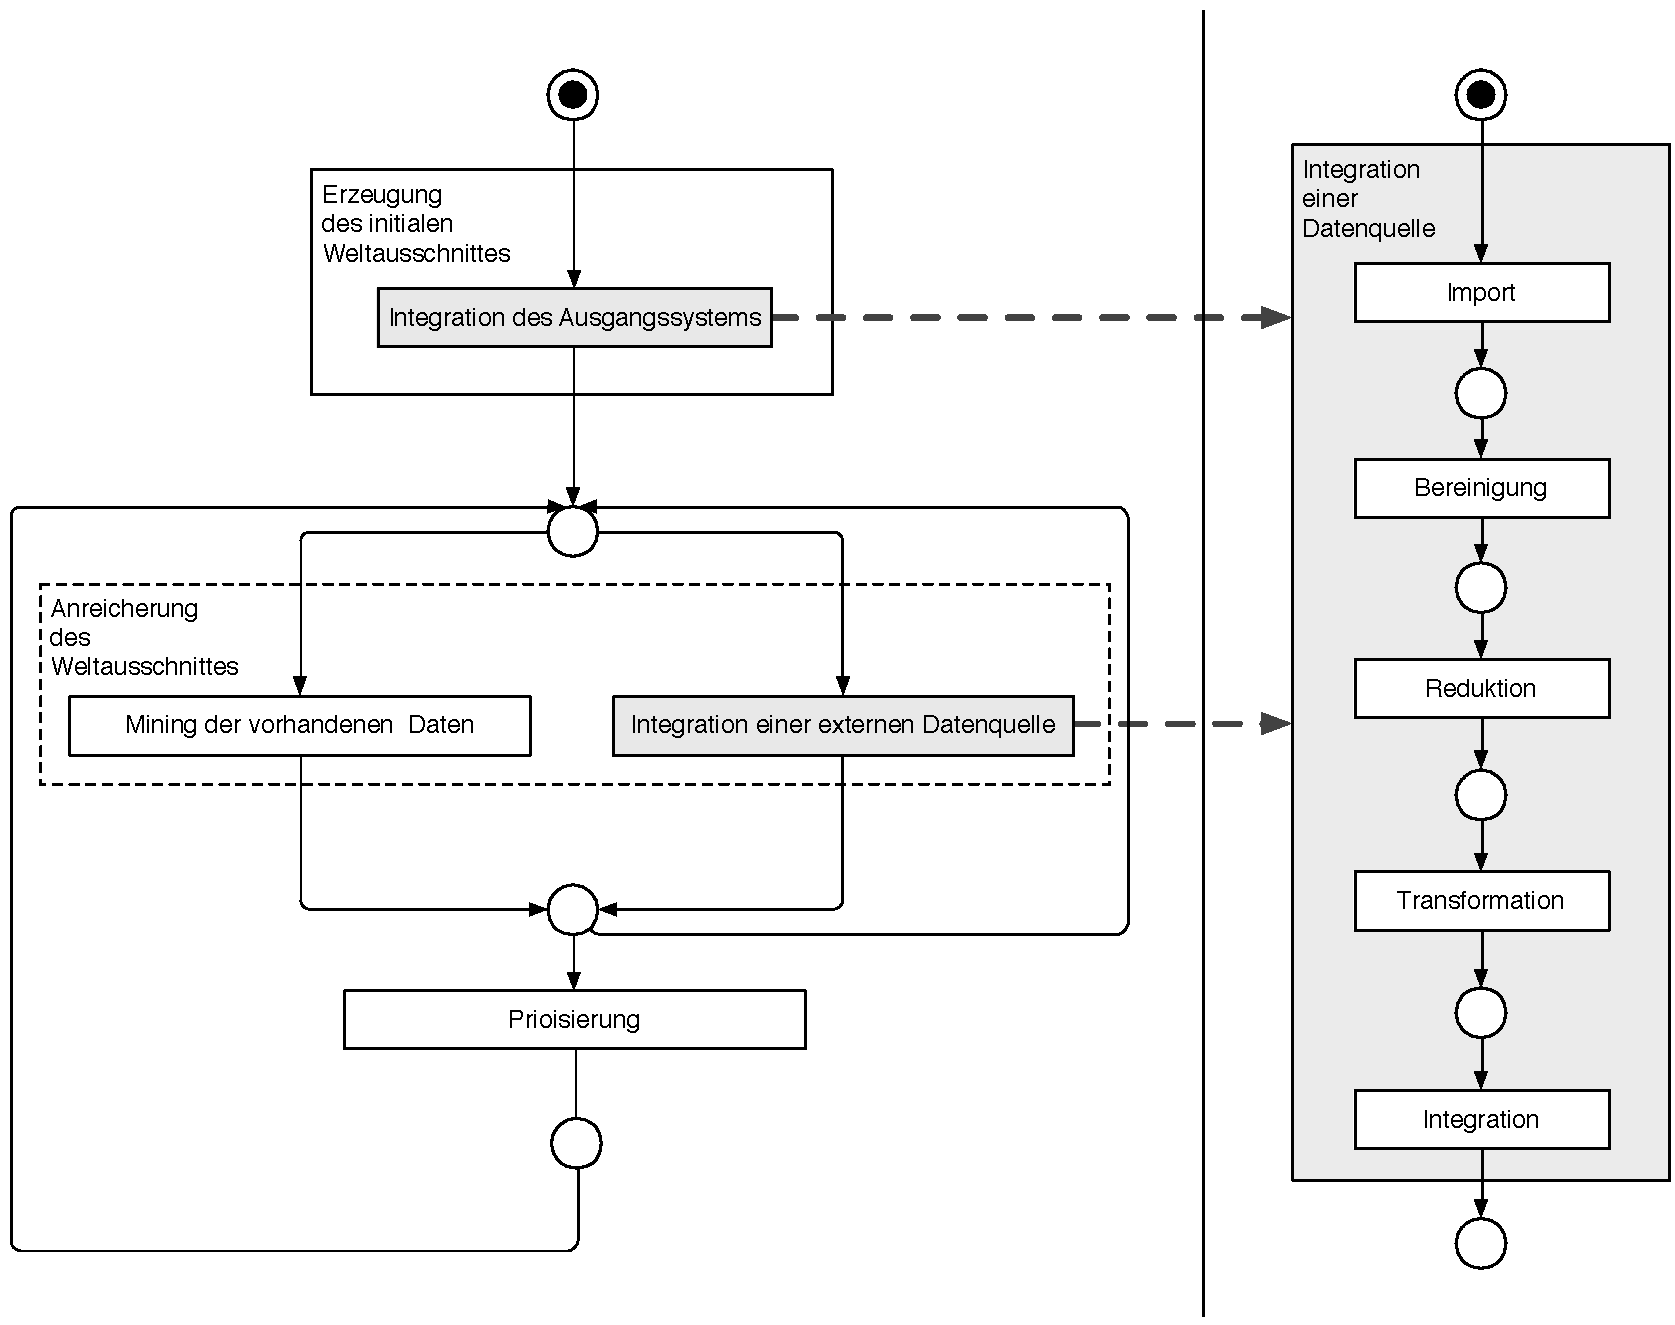
\includegraphics[width=\textwidth]{link_discovery_process}
\caption{Link--Discovery--Prozess als Petrinetz}
\label{fig:link_discovery_process}
\end{figure}

Die grundlegenden Phasen des Prozesses sind die \emph{Erzeugung} des initialen Weltausschnittes, dessen \emph{Anreicherung} und die \emph{Prioisierung} der Beziehungen. Sowohl bei der initialen Erzeugung, als auch bei der Anreicherung wird ein Prozess zur Integration von Datenquellen benötigt.

Die Schritte der Anreicherung und Priosierung können beliebig oft wiederholt werden, um das Ergebnis zu verbessern und auf die gewünschte Anwendung anzupassen. Die Anreicherung kann grundsätzlich durch das Mining der bereits im Weltausschnitt vorhandenen Daten oder durch die Integration neuer Datenquellen erfolgen.

Die genannten Schritte werden in den folgenden Abschnitten erläutert.